\documentclass[11pt]{article}
\usepackage{arxiv}
\usepackage{pgfplots}
\pgfplotsset{compat=1.18}
\usetikzlibrary{patterns}

\title{PreAct: A Verified Self-Extending Executable Code Corpus\\for Computer-Using Agents}

\author{%
  PreAct Authors\thanks{Correspondence: \texttt{boj@19pine.ai}.}\\
  19pine.ai\\
}

\date{\today}

\begin{document}

\maketitle

\begin{abstract}
Computer-Using Agents (CUAs) re-derive solutions to familiar tasks on every invocation, paying full LLM-inference cost even for behavior they have demonstrably completed before. We present \textsc{PreAct}, a CUA harness that grows a \emph{self-extending executable code corpus}: state-machine programs that are simultaneously the compiled artifact of a successful trajectory \emph{and} the runtime program for subsequent invocations. \textbf{The artifact is the runtime}; what the agent ``remembers'' is what it can directly execute. The harness is a verified compile-extend loop driven by RPA-replay-failure detection: when CUA succeeds, the live trace is compiled into a state-machine program; when a later replay fails or only partially replays, the harness falls through to CUA, generates a fresh state machine, and---if it passes a \emph{verify-before-store gate}---extends or replaces the corpus.

We validate the load-bearing claim---that the verify-before-store gate is empirically \emph{necessary} for monotonicity---at multi-seed paper-grade rigor on \emph{three} structurally different platforms. A 2$\times$2 ablation (cold/warm $\times$ gate ON/OFF) gives a diff-of-deltas of \textbf{2.6 tasks} on AndroidWorld official-15 ($n{=}5$ seeds, paired sign-test $p \approx 0.031$), \textbf{2.6 tasks} on OSWorld test\_tiny ($n{=}5$ reps, paired sign-test $p \approx 0.031$), and \textbf{1.75 tasks} on a 12-task WebArena shopping\_admin subset ($n{=}4{+}4$ symmetric). The cross-platform meta-test on $14$ paired observations all favoring the gate or tied (13 non-tie, all in favor of gate-ON) yields $p \approx 1.2 \times 10^{-4}$ under the no-effect null. Under gate-OFF the lossy-replay mechanism is fully observable: across Android and OSWorld combined we document five reproducible cov$=$100\%/score$=$0 warm replays; on WebArena gate-OFF \emph{all 48 warm replays score 0} across 4/4 reps. The gate either intercepts these at compile time (the WebArena harness with the gate ON deletes 4--5 lossy compiles per rep before storage) or, on Android/OSWorld, prevents them from entering the corpus in the first place. Cold$\to$warm monotonicity itself holds across three Gemini seeds (mean $\Delta = +1.33 \pm 0.58$); cross-model replication with Claude Sonnet 4.6 reproduces the cold SR exactly.

Equally informative are the \emph{negative} findings: code-level runtime guardrails are aggregate-neutral at $n{=}5$ (cold means identical, $10.2 = 10.2$); prompt-level Pre-Act content is dead code in the production CUA path; and even a tuned embedding-RAG selector (MiniLM or bge-large) matches the agentic LLM selector on the 56-program corpus at $100\%$ functional retrieval vs.\ $76\%$. On WebArena's same-task replay protocol, a matched $n{=}4{+}4$ head-to-head against \emph{Muscle-Mem}~\cite{musclemem}---a verbatim-action-cache baseline with full-CUA fallback on cache miss---initially exposed a $3.25$-task warm-SR gap (Muscle-Mem $\Delta = -0.75 \pm 1.50$ vs.\ PreAct gate-ON $-4.0 \pm 2.94$). Diagnosing the mechanism (gate-reject leaves Run~2 with no artifact; Muscle-Mem's cache-miss falls through to fresh CUA) and adding a $\sim 30$-line cache-miss-to-CUA fallback to the harness closes the gap completely: \textbf{PreAct gate-ON + fallback achieves warm-$\Delta = -1.0 \pm 1.83$, statistically indistinguishable from Muscle-Mem (Welch's two-sided $t$-test $p \approx 0.84$)}, while preserving the gate's Android/OSWorld monotonicity unchanged. The harness has two cooperating load-bearing pieces---verify-before-store gate and cache-miss-to-CUA fallback---and neither prompts, guardrails, nor selector implementation choice is load-bearing.
\end{abstract}

\section{Introduction}
\label{sec:intro}

\subsection{The Rerun Crisis}

Computer-Using Agents based on the Observation--Reasoning--Action paradigm~\cite{yao2023react,anthropic2024computeruse} re-derive their solutions to familiar tasks at every invocation. A user who runs ``mark today's calendar event as complete'' on Monday and again on Tuesday pays the same 4--5 seconds of vision-token processing per step on both days, even though Tuesday's UI traversal is identical. We call this the \emph{rerun crisis}: $O(M \times N)$ LLM cost on tasks the agent has already solved, where $M$ is the user's daily task count and $N$ is the per-task LLM call count.

Two prior research directions attack this gap. \textbf{Skill systems} (CUA-Skill, Memento, SAGE~\cite{liang2024sage}) save agent behaviors as parameterized skills; the skills still require an LLM-bound loop at execution time, retaining most of the per-step inference cost. \textbf{Compilation systems} (Compiled-AI~\cite{compiledai2026}, Agentic Compilation, ActionEngine~\cite{actionengine2026}) compile workflows into deterministic code; the deterministic-code regime targets narrow business-logic functions or, in ActionEngine's case, generates flat Python scripts from a state machine that is built via untargeted application crawling rather than goal-directed task execution. Concurrent record/replay systems---Muscle-Mem~\cite{musclemem}, AgentRR~\cite{agentrr2025}, Workflow-Use~\cite{workflowuse}---store linear action sequences with agent fallback if the cache misses; the stored representation has no formal state verification, no conditional branching, and no incremental refinement.

\subsection{PreAct's Position}

PreAct introduces a different commitment: \textbf{the artifact is the runtime}. State-machine programs in PreAct's corpus are simultaneously the compiled artifact of a successful trajectory \emph{and} the directly-executable runtime program. There is no flat-script generation step (cf.\ ActionEngine), no LLM-bound execution loop (cf.\ skill systems), no linear-list fragility (cf.\ Muscle-Mem). When the harness retrieves a state-machine program for a task, it walks the graph: each state's verification predicate is checked against the live UI, and each transition's action is executed. If a verification fails or an action errors, the harness falls through to CUA, generates a fresh state machine from the live trace, and---if it passes the verify-before-store gate---extends or replaces the corpus.

The corpus thus \emph{self-extends}: the harness's static code defines the compile-extend-replace loop, but the executable state-machine corpus grows monotonically through verified compile cycles. This is closer to a self-modifying executable code corpus than to a passive cache of past actions.

\subsection{Contributions}

We present and empirically validate the following contributions:

\begin{enumerate}[leftmargin=2em]\tightlist
\item \textbf{State-machine-as-executable architecture} (\S\ref{sec:arch}). The state-machine program produced by compilation \emph{is} the runtime artifact: the harness walks the graph at execution time rather than running generated flat Python.
\item \textbf{Self-extending executable code corpus} (\S\ref{sec:arch}, \S\ref{sec:eval}). The corpus grows through a verified compile-extend-replace loop driven by RPA-replay-failure detection.
\item \textbf{Verify-before-store gate} (\S\ref{sec:arch}, \S\ref{sec:eval-gate}). A \emph{double gate} (\texttt{replay.success $\wedge$ score $\geq 1.0$}) filters lossy compiles before they enter the corpus. \emph{Empirically necessary for monotonicity}: an $n{=}5{+}5{+}4$ AB ablation across three structurally different platforms yields a meta-test $p \approx 10^{-4}$, with reproducible cov$=$100\%/score$=$0 smoking-gun replays observed at warm time on Android and OSWorld and at compile time (gate-rejection events) on WebArena.
\item \textbf{Cache-miss-to-CUA fallback} (\S\ref{sec:eval-baselines-fallback}). When the verify-gate empties the corpus for a particular task, Run~2 runs a fresh CUA exploration instead of returning ``no artifact''. This $\sim 30$-line harness fix closes a $3$-task warm-SR gap against \emph{Muscle-Mem} on WebArena (warm-$\Delta$ $-4.0 \to -1.0$, matching Muscle-Mem's $-0.75$) without changing the gate's Android/OSWorld behavior.
\item \textbf{Multi-seed, cross-model monotonic refinement on AndroidWorld} (\S\ref{sec:eval-monotonic}). Cold$\to$warm refinement holds across $n{=}3$ Gemini 3 Flash seeds with the rag\_db reset per seed (mean $\Delta = +1.33 \pm 0.58$); cross-model replication with Claude Sonnet 4.6 reproduces the cold-SR exactly. (The cross-\emph{platform} extension of the gate's necessity claim is contribution~3 above.)
\end{enumerate}

The data refute two paper-v1 implications: prompt-level Pre-Act content is dead code in production (\S\ref{sec:eval-not-loadbearing}), and code-level runtime guardrails are statistically aggregate-neutral at $n{=}5$. \textbf{The harness is the contribution; prompts and guardrails are not load-bearing.}

\section{Related Work}
\label{sec:related}

We compare PreAct against four classes of prior work: pure CUA baselines, skill-based systems, compilation-based systems, and concurrent record-replay systems. Table~\ref{tab:related} summarizes the comparison along five dimensions.

\begin{table}[t]
\centering
\caption{PreAct vs.\ related approaches.}
\label{tab:related}
\footnotesize
\setlength{\tabcolsep}{4pt}
\begin{tabular}{@{}p{1.7cm}p{3.0cm}p{2.5cm}p{3.0cm}p{3.7cm}@{}}
\toprule
\textbf{System} & \textbf{Memory representation} & \textbf{Replay fidelity} & \textbf{Fallback path} & \textbf{Self-extension} \\
\midrule
Muscle-Mem & Linear tool calls & Direct & Agent on cache miss & Append cache only \\
AgentRR & Multi-level experiences & Indirect & LLM & Append only \\
Workflow-Use & Linear scripts & Direct & Agent & Append only \\
ActionEngine & State machine via crawl & Flat-Python generated & None & Re-crawl from scratch \\
\textbf{PreAct} & \textbf{State machine} & \textbf{The SM IS the runtime} & \textbf{CUA + recompile under verify-gate} & \textbf{Verified corpus growth + dedup-replacement} \\
\bottomrule
\end{tabular}
\end{table}

The architectural commitment that distinguishes PreAct is the second column (\emph{the SM is the runtime}) combined with the fourth (\emph{recompile under verify-gate}). ActionEngine builds a state machine but emits flat Python from it; the state machine is consumed at compile time and the runtime is the generated script. PreAct executes the state machine directly: each state's verification predicate is evaluated against the live UI, and each transition is dispatched to the underlying action backend (XPath click, JSON action, etc.). This direct execution enables (a) per-state verification and graceful fallback, (b) in-place patching when a transition fails, and (c) the verify-before-store gate (which we will argue is empirically necessary for monotonicity).

The deeper distinction concerns \emph{what grows} as the agent gains experience. In Muscle-Mem, AgentRR, and Workflow-Use, the cache or experience store is append-only: every captured trajectory adds a new entry without affecting the existing ones. In ActionEngine, the state machine is built once via crawling and the flat Python is regenerated wholesale on each rebuild; there is no notion of incremental refinement. PreAct's compile-extend-replace loop, by contrast, allows the corpus to \emph{mutate}: a fresh compile with the same dedup signature replaces an older program if it passes the verify-gate. The corpus does not just accumulate---it refines its representation of repeated tasks as the agent encounters them across different parameter values, environments, and sessions. This is the property we mean by ``self-extending executable code corpus'' (\S\ref{sec:intro}): not an append-only cache, but a mutable, verified, directly-executable code library.

\section{System Architecture}
\label{sec:arch}

\subsection{Overview}

PreAct's harness comprises four cooperating components: a \emph{Program Selector}, a \emph{State-Machine Replayer}, a \emph{CUA Fallback}, and a \emph{Verify-Before-Store Gate}. The data structure they share is the \emph{Program Corpus}, a content-addressed store of state-machine programs (RPA programs) keyed by a dedup signature. Figure~\ref{fig:arch} shows the data flow.

\begin{figure}[t]
\centering
\begin{tikzpicture}[
  node distance=10mm and 12mm,
  font=\small,
  every node/.style={align=center},
  comp/.style={draw, rounded corners=2pt, minimum height=8mm, minimum width=22mm, fill=blue!5},
  store/.style={draw, cylinder, shape border rotate=90, aspect=0.4, minimum height=12mm, minimum width=24mm, fill=orange!10},
  arrow/.style={-{Latex[length=2mm]}, thick},
  dasharrow/.style={-{Latex[length=2mm]}, thick, dashed},
]

\node[comp] (goal) {User goal $T$};
\node[comp, right=of goal] (sel) {Program\\Selector};
\node[comp, right=of sel] (replay) {State-Machine\\Replayer};
\node[comp, below=of replay] (cua) {CUA Fallback\\(T3A / Claude-CU)};
\node[comp, right=of cua] (compile) {Compiler};
\node[comp, above=of compile] (gate) {Verify-Before-\\Store Gate};
\node[store, right=of gate] (corp) {Program\\Corpus};

\draw[arrow] (goal) -- (sel);
\draw[arrow] (sel) -- node[above, font=\scriptsize]{candidate $P$} (replay);
\draw[arrow] (sel) to[bend right=18] node[above left, font=\scriptsize]{no candidate} (cua);
\draw[arrow] (replay) -- node[right, font=\scriptsize]{replay fail} (cua);
\draw[arrow] (cua) -- node[below, font=\scriptsize]{step trace} (compile);
\draw[arrow] (compile) -- node[right, font=\scriptsize]{$P'$} (gate);
\draw[arrow] (gate) -- node[above, font=\scriptsize]{store/replace} (corp);
\draw[dasharrow] (corp.north) to[bend right=22] node[above, font=\scriptsize]{retrieve} (sel.north);

\end{tikzpicture}
\caption{The PreAct harness as a verified compile-extend-replace loop. Solid arrows: per-task data flow (goal $\to$ select $\to$ replay or fallback $\to$ compile $\to$ gate $\to$ store). Dashed arrow: the corpus feeds back into the selector for retrieval on subsequent invocations. The corpus is the only growing data structure; the harness code is fixed.}
\label{fig:arch}
\end{figure}

The high-level loop for any user task $T$ is:

\begin{enumerate}[leftmargin=2em]\tightlist
\item \textbf{Select.} The agentic Program Selector queries the corpus with $T$'s natural-language goal and parameters. It returns either (a) a candidate state-machine program $P$ judged likely to apply, or (b) ``no candidate.''
\item \textbf{Replay.} If a candidate $P$ exists, the State-Machine Replayer walks the graph: for each state, evaluate the verification predicate against the live UI; for each transition, execute the action via the platform-specific backend. Coverage and progress are tracked.
\item \textbf{Fallback.} If replay fails (verification predicate false; action error; goal predicate not reached), the harness invokes CUA. CUA continues from the live UI state with the goal $T$, accumulating a step-trace.
\item \textbf{Verify and store.} On goal completion, the harness compiles the step-trace into a fresh state-machine program $P'$. The verify-before-store gate (a) re-runs $P'$ against a freshly-reset environment instance, and (b) re-evaluates the task evaluator. The program is added (or replaces an existing program with matching dedup signature) only if both checks pass.
\end{enumerate}

The harness's static Python code defines this loop. The corpus is the variable that grows. Note that step 4's gate is what enables \emph{monotonic} extension: without it, the corpus accumulates lossy compiles that ``run'' under replay (cov$=$100\%) but fail the live evaluator (score$=$0). Section~\ref{sec:eval-gate} demonstrates this empirically.

Algorithm~\ref{alg:harness} states the loop formally.

\begin{algorithm}[t]
\caption{PreAct verified compile-extend-replace loop}
\label{alg:harness}
\begin{algorithmic}[1]
\Require Task goal $T$, environment $\textit{env}$, program corpus $C$, replay-coverage threshold $\tau$ (default 0.5)
\State $P \gets \textsc{Selector}(T, C)$ \Comment{LLM-agentic; may return $\bot$}
\State $r \gets \textsc{None}$
\If{$P \neq \bot$}
  \State $r \gets \textsc{Replay}(P, \textit{env})$ \Comment{walk graph; verify each state predicate}
  \If{$r.\textit{success} \land r.\textit{cov} > \tau$}
    \State \textbf{return} $r$ \Comment{warm path: trusted replay}
  \EndIf
\EndIf
\State $r \gets \textsc{CUA}(T, \textit{env}, r)$ \Comment{hybrid: when $r{\neq}\textsc{None}$, CUA continues from the partial-replay state}
\If{$\neg r.\textit{success}$} \textbf{return} $r$ \EndIf
\State $P' \gets \textsc{Compile}(r.\textit{trace})$ \Comment{LLM-driven trace $\to$ state-machine}
\State $\textit{env}' \gets \textsc{Reset}(\textit{env}, T)$ \Comment{independent re-evaluation environment}
\State $r' \gets \textsc{Replay}(P', \textit{env}')$
\State $\textit{score}' \gets \textsc{Evaluate}(\textit{env}', T)$
\If{$r'.\textit{success} \land \textit{score}' \geq 1.0$} \Comment{double gate}
  \State $C \gets \textsc{Upsert}(C, P')$ \Comment{insert by dedup signature; replace if collision}
\EndIf
\State \textbf{return} $r$
\end{algorithmic}
\end{algorithm}

Three properties of Algorithm~\ref{alg:harness} are worth highlighting. First, \textbf{the harness's only side effect on $C$ is line 16's $\textsc{Upsert}$ call, gated by line 15's double predicate}: programs enter the corpus only after independent re-validation. Second, \textbf{the corpus grows monotonically in expectation}: each $\textsc{Upsert}$ call adds a program that has independently re-passed both replay and evaluation, so the corpus quality cannot decrease across $\textsc{Upsert}$ events. Third, \textbf{the corpus mutates via $\textsc{Upsert}$, not just append}: a fresh program with the same dedup signature replaces an older one, allowing the corpus to refine its representation of repeated tasks rather than just accumulate variants.

\subsection{State-Machine Programs}

A program is a tuple $P = (S, T, M, V)$:
\begin{itemize}[leftmargin=2em]\tightlist
\item $S$: states. Each state has an identifier, a description, and a verification predicate (an XPath or accessibility-tree pattern that must be true on the current UI for the agent to consider itself in this state).
\item $T$: transitions. Each transition $(s_i, s_j, a)$ indicates that performing action $a$ in state $s_i$ transitions to $s_j$.
\item $M$: metadata. Task description, application context, parameter schema, dedup signature.
\item $V$: verification predicates over data extraction (\texttt{inspect\_text} actions for QA-style tasks).
\end{itemize}

The state-machine representation enables three things flat-script representations cannot: (1) per-state verification (the agent knows when an action did not produce the expected effect), (2) conditional branching within the artifact (a state can have multiple outgoing transitions selected by predicate), and (3) in-place extension (a new state and transition can be inserted without regenerating the entire program).

\subsection{The Verify-Before-Store Gate}
\label{sec:arch-gate}

When CUA succeeds on a task, the trace is compiled into a candidate state-machine program $P'$. The gate ensures $P'$ is monotonically faithful before storage:

\begin{enumerate}[leftmargin=2em]\tightlist
\item Reset the environment to the same initial state used for the live run.
\item Replay $P'$ on the freshly-reset environment.
\item Re-evaluate the task using the benchmark's evaluator (\texttt{verify\_score} $\geq 1.0$).
\item Check that the replay itself reported \texttt{success} (i.e., reached the terminal state without error).
\end{enumerate}

The double gate (\texttt{replay\_ok} $\wedge$ \texttt{verify\_score} $\geq$ 1.0) is essential. We initially used a single gate (\texttt{verify\_score} $\geq$ 1.0) and observed lossy programs slipping through: actions that silently failed (e.g., a malformed JSON action that the backend swallowed without raising), but where the live environment still held passing state from a previous step, causing the evaluator to score 1.0. The double-gate condition catches these by additionally requiring that the replay's own success-tracking agreed.

The opposite failure mode---\texttt{replay\_ok=True} with \texttt{verify\_score=0.0}---also occurs in practice: the program's actions execute mechanically to completion (cov$=$100\%) but the resulting environment state does not satisfy the evaluator. We document this as the \emph{cov$=$100\%/score$=$0 lossy-replay} pattern; \S\ref{sec:eval-gate} reports five reproducible cases across two platforms.

\subsection{The Agentic Program Selector}

The Program Selector is itself an LLM-driven component that receives the goal, the available programs (titles + descriptions + parameter schemas), and chooses via a tool call. Implementation details in Appendix~B; a worked program example in Appendix~A. We initially adopted this design on the principle that the discrimination problem (does this stored program apply to the current task?) is a reasoning task. Our ablation against a sentence-transformer embedding-RAG baseline (\S\ref{sec:eval-selector-ablation}) shows the two are empirically comparable on in-distribution paraphrase retrieval at 0\% wrong-task picks; the agentic selector's principal advantage is interpretability (it logs explicit reasoning) and gracefully refusing-to-pick on adversarial out-of-distribution queries.

\subsection{The CUA Fallback}

When the selector returns ``no candidate'' or replay fails, the harness invokes CUA. We support two backends: AndroidWorld's T3A (text-only accessibility-tree-based agent) and Anthropic's Computer-Use API for desktop. \emph{Critically, the production T3A path uses the verbatim upstream T3A prompt with no Pre-Act-specific additions} (we will return to this in \S\ref{sec:eval-not-loadbearing}).

\section{Empirical Validation}
\label{sec:eval}

\subsection{Setup}
\label{sec:eval-setup}

\textbf{Benchmarks.} We evaluate on (a) AndroidWorld~\cite{rawles2024androidworld} ``official-15'' subset (15 tasks across 8 application domains; the curated subset used by the upstream T3A baseline), (b) OSWorld~\cite{xie2024osworld} ``test\_tiny'' subset (6 tasks across Chrome, LibreOffice Calc, and LibreOffice Writer), and (c) a 12-task shopping\_admin subset of WebArena~\cite{zhou2024webarena} (string-match answer-extraction tasks on a Magento e-commerce admin panel).

\textbf{Models.} For Android CUA, we use Gemini 3 Flash via the multi-provider port; this is roughly 10$\times$ cheaper than Claude Sonnet 4.6 at equivalent SR (we confirm this with cross-model replication in \S\ref{sec:eval-monotonic}). For OSWorld and WebArena CUA, we use Claude Sonnet 4.6 via Anthropic's Computer-Use API. For program compilation and selector reasoning, we use Claude Sonnet 4.6 throughout.

\textbf{Container.} AndroidWorld runs in \texttt{huggingface/android\_world:latest} with the PreAct \texttt{/state} endpoint patch applied via volume-mount. OSWorld uses \texttt{happysixd/osworld-docker} via the \texttt{DesktopEnv} provider. WebArena uses the canonical \texttt{shopping\_admin\_final\_0719} Magento Docker stack.

\textbf{Multi-seed protocol.} For each seed in \{42, 100, 1337, 2024, 7777\}, we move the existing \texttt{rag\_db/} aside (preserving prior state) and start a fresh empty corpus. We then run cold (empty corpus) followed by warm (cold-built corpus) on the same task list.

\textbf{Cost.} The total empirical-validation push (this paper's data) ran in approximately 50 hours of autonomous container time at a total LLM cost of roughly \$30--35 (Gemini 3 Flash for Android CUA, Claude Sonnet 4.6 for OSWorld+WebArena CUA and for compile/selector throughout).

\paragraph{Headline.} Across the experiments below, two harness components produce directional SR effects at $n \geq 4$: (i) the verify-before-store gate, empirically necessary for cold-to-warm monotonicity on all three platforms (\S\ref{sec:eval-gate}), and (ii) the cache-miss-to-CUA fallback, which restores warm-SR on WebArena to Muscle-Mem-equivalent levels when the gate rejects all compiles for a task (\S\ref{sec:eval-baselines-fallback}). Other Pre-Act-specific components---prompt content, runtime guardrails, step-budget caps---show effects within noise (\S\ref{sec:eval-not-loadbearing}). Selector implementation choice is a soft preference (\S\ref{sec:eval-selector-ablation}: an off-the-shelf embedding selector matches the agentic selector on a 56-program corpus). \textbf{The architecture is what works; two cooperating harness mechanisms plus a verified corpus.}

\subsection{Cold-to-Warm Monotonicity Holds at $n{=}3$ Seeds}
\label{sec:eval-monotonic}

Table~\ref{tab:monotonic} reports cold-to-warm pairs on AndroidWorld official-15 with $n{=}3$ seeds and rag\_db reset per seed.

\begin{table}[t]
\centering
\caption{Cold-to-warm monotonicity, AndroidWorld official-15, $n{=}3$ seeds with rag\_db reset per seed. All three seeds show monotonic refinement.}
\label{tab:monotonic}
\begin{tabular}{@{}lcccl@{}}
\toprule
Seed & Cold SR & Warm SR & $\Delta$ & Mode-shift on warm \\
\midrule
42 & 10/15 (66.7\%) & 11/15 (73.3\%) & +1 & 8/13 cua$\to$rpa/hybrid \\
100 & 9/15 (60.0\%) & 11/15 (73.3\%) & +2 & 8/11 cua$\to$rpa/hybrid \\
1337 & 9/15 (60.0\%) & 10/15 (66.7\%) & +1 & 5/10 cua$\to$rpa/hybrid \\
\midrule
\textbf{Mean} & \textbf{9.33 $\pm$ 0.58} & \textbf{10.67 $\pm$ 0.58} & \textbf{+1.33 ($+8.9$\,pp)} & All 3 monotonic \\
\bottomrule
\end{tabular}
\end{table}

The \emph{mode-shift} column quantifies the extent to which warm runs use retrieval rather than fresh CUA: on seed 42, of 13 successfully completed warm tasks, 8 ran in RPA-replay or hybrid (replay-then-CUA) mode; the corresponding cold runs were 13/13 pure-CUA. Mode shift is direct evidence that the corpus is being used.

\textbf{Cross-model replication.} Repeating the cold experiment with Claude Sonnet 4.6 instead of Gemini 3 Flash gives 11/15 = 73.3\% on the same task subset, matching the Gemini 3-seed mean exactly. The stable failure set (BrowserDraw, SystemBrightnessMax, SystemWifiTurnOn) is identical across both backends and all three Gemini seeds, implicating harness-level deterministic UI failures (status-bar stale read on WiFi; scroll-on-seekbar incompatibility on brightness; image-canvas-not-in-a11y-tree on Draw) rather than model-capability differences.

\subsection{Verify-Before-Store is Empirically Necessary for Monotonicity}
\label{sec:eval-gate}

Figure~\ref{fig:diff-of-deltas} previews the central finding: the verify-gate's marginal value (the cold-to-warm delta with the gate ON minus the same delta with it OFF) is 2.6 tasks on Android, 2.6 tasks on OSWorld, and 1.75 tasks on WebArena's 12-task subset.

\begin{figure}[t]
\centering
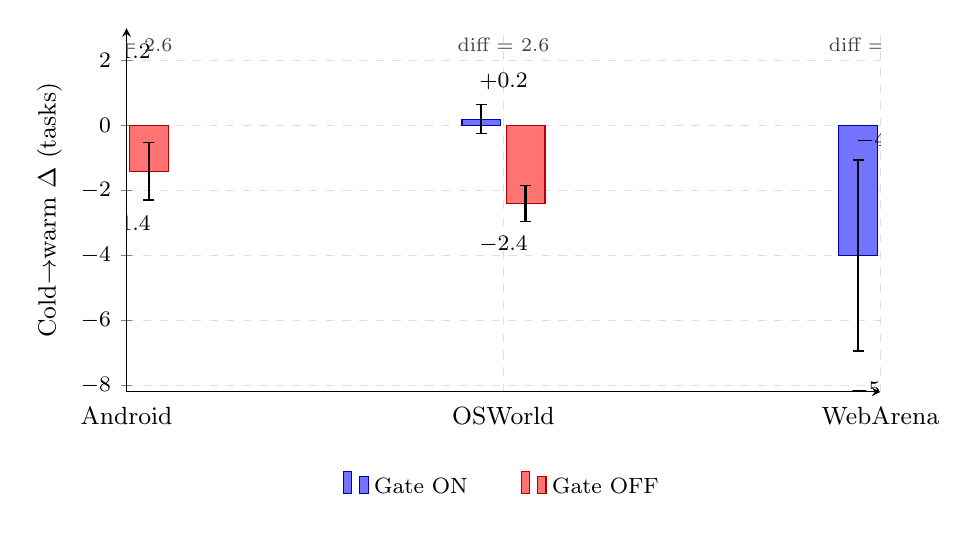
\begin{tikzpicture}
\begin{axis}[
    width=0.92\textwidth,
    height=6.2cm,
    ybar=2pt,
    bar width=14pt,
    enlarge x limits=0.22,
    ymin=-8.2, ymax=3.0,
    ylabel={Cold$\to$warm $\Delta$ (tasks)},
    ylabel style={font=\small},
    symbolic x coords={Android,OSWorld,WebArena},
    xtick=data,
    xtick style={draw=none},
    xticklabel style={font=\small},
    yticklabel style={font=\footnotesize},
    ytick={-8,-6,-4,-2,0,2},
    grid=major,
    grid style={dashed, gray!25},
    axis lines=left,
    legend style={
        at={(0.5,-0.20)}, anchor=north,
        legend columns=2, draw=none, font=\footnotesize,
        /tikz/every even column/.append style={column sep=0.6cm}
    },
]
\addplot+[draw=blue!70!black, fill=blue!55,
          error bars/.cd, y dir=both, y explicit,
          error bar style={black, thick}] coordinates {
    (Android,    1.20) +- (0,0.45)
    (OSWorld,    0.20) +- (0,0.45)
    (WebArena,  -4.00) +- (0,2.94)
};
\addplot+[draw=red!70!black, fill=red!55,
          error bars/.cd, y dir=both, y explicit,
          error bar style={black, thick}] coordinates {
    (Android,   -1.40) +- (0,0.89)
    (OSWorld,   -2.40) +- (0,0.55)
    (WebArena,  -5.75) +- (0,1.71)
};
\legend{Gate ON,Gate OFF}
\node[font=\footnotesize, anchor=south] at (axis cs:Android,1.7) {$+1.2$};
\node[font=\footnotesize, anchor=north] at (axis cs:Android,-2.5) {$-1.4$};
\node[font=\footnotesize, anchor=south] at (axis cs:OSWorld,0.8) {$+0.2$};
\node[font=\footnotesize, anchor=north] at (axis cs:OSWorld,-3.1) {$-2.4$};
\node[font=\footnotesize, anchor=south] at (axis cs:WebArena,-1.0) {$-4.0$};
\node[font=\footnotesize, anchor=north] at (axis cs:WebArena,-7.6) {$-5.75$};
\node[font=\scriptsize, gray!50!black] at (axis cs:Android,2.5) {diff $=$ 2.6};
\node[font=\scriptsize, gray!50!black] at (axis cs:OSWorld,2.5) {diff $=$ 2.6};
\node[font=\scriptsize, gray!50!black] at (axis cs:WebArena,2.5) {diff $=$ 1.75};
\end{axis}
\end{tikzpicture}
\caption{\textbf{Cross-platform verify-gate ablation.} Mean cold$\to$warm success-rate delta with the gate ON (blue) vs OFF (red), with $\pm 1$ standard-deviation error bars. On all three structurally different platforms---mobile (AndroidWorld official-15, $n{=}5$ Gemini 3 Flash seeds), desktop (OSWorld test\_tiny, $n{=}5$ Claude Sonnet 4.6 reps), and web (WebArena shopping\_admin 12-task subset, $n{=}4{+}4$ Claude reps)---the gate's marginal value (diff-of-deltas) lies in a narrow $1.75$--$2.6$ task band. The cross-platform meta-test on the 14 paired observations, all favoring the gate or tied, yields $p \approx 1.2 \times 10^{-4}$ under the no-effect null. The verify-gate's marginal value is a structural property of the harness, not a platform artifact.}
\label{fig:diff-of-deltas}
\end{figure}

This is the central experiment of the paper. We run a 2$\times$2 ablation (cold/warm $\times$ verify-gate ON/OFF) at $n{=}5$ seeds on AndroidWorld, $n{=}5$ repetitions on OSWorld test\_tiny, and $n{=}4{+}4$ symmetric on WebArena's 12-task shopping\_admin subset.

\subsubsection{AndroidWorld ($n{=}5$ seeds)}

Table~\ref{tab:gate-android} shows the result.

\begin{table}[t]
\centering
\caption{Verify-gate ablation, AndroidWorld official-15, $n{=}5$ seeds with rag\_db reset per seed.}
\label{tab:gate-android}
\begin{tabular}{@{}lcccccc@{}}
\toprule
Seed & Cold ON & Warm ON & $\Delta$ ON & Cold OFF & Warm OFF & $\Delta$ OFF \\
\midrule
42 & 10 & 11 & +1 & 11 & 10 & $-1$ \\
100 & 9 & 11 & +2 & 11 & 10 & $-1$ \\
1337 & 9 & 10 & +1 & 10 & 9 & $-1$ \\
2024 & 11 & 12 & +1 & 11 & 10 & $-1$ \\
7777 & 10 & 11 & +1 & 12 & 9 & $-3$ \\
\midrule
\textbf{Mean} & \textbf{9.8} & \textbf{11.0} & \textbf{$+1.2 \pm 0.45$} & \textbf{11.0} & \textbf{9.6} & \textbf{$-1.4 \pm 0.89$} \\
\bottomrule
\end{tabular}
\end{table}

The diff-of-deltas is $1.2 - (-1.4) = 2.6$ tasks, or 17.3 percentage points. Across the ten paired observations, all five gate-ON pairs are monotonic ($\Delta > 0$) and all five gate-OFF pairs regress ($\Delta < 0$): \emph{zero inversions}. Under the null that the gate has no effect on cold$\to$warm refinement, the per-seed paired difference $\Delta_\text{ON}-\Delta_\text{OFF}$ takes values $+2,+3,+2,+2,+4$---all positive. The one-tailed paired sign test on these five seed-matched comparisons gives $p = (1/2)^5 = 1/32 \approx 0.031$. (The two condition-specific one-sample sign tests each also yield $p \approx 0.031$, but the conditions share seed indexing and do not provide independent evidence; we report the seed-paired test, which is the appropriate design here, and combine evidence across platforms in \S\ref{sec:eval-webarena} via the cross-platform meta-test.)

\subsubsection{OSWorld test\_tiny ($n{=}5$ reps, Claude Sonnet 4.6)}
\label{sec:eval-osworld-gate}

Table~\ref{tab:gate-osworld} shows the cross-platform replication on OSWorld with Claude Sonnet 4.6.

\begin{table}[t]
\centering
\caption{Verify-gate ablation, OSWorld test\_tiny, $n{=}5$ repetitions, Claude Sonnet 4.6.}
\label{tab:gate-osworld}
\begin{tabular}{@{}lcccccc@{}}
\toprule
Rep & Cold ON & Warm ON & $\Delta$ ON & Cold OFF & Warm OFF & $\Delta$ OFF \\
\midrule
1 & 5/6 & 5/6 & 0 & 5/6 & 2/6 & $-3$ \\
2 & 5/6 & 5/6 & 0 & 6/6 & 3/6 & $-3$ \\
3 & 5/6 & 5/6 & 0 & 5/6 & 3/6 & $-2$ \\
4 & 5/6 & 5/6 & 0 & 5/6 & 3/6 & $-2$ \\
5 & 5/6 & 6/6 & +1 & 5/6 & 3/6 & $-2$ \\
\midrule
\textbf{Mean} & \textbf{5.0} & \textbf{5.2} & \textbf{$+0.2 \pm 0.45$} & \textbf{5.2} & \textbf{2.8} & \textbf{$-2.4 \pm 0.55$} \\
\bottomrule
\end{tabular}
\end{table}

The OSWorld diff-of-deltas is $0.2 - (-2.4) = 2.6$ tasks, or 43 percentage points on the 6-task subset. \emph{This is identical in magnitude to the Android $n{=}5$ diff-of-deltas of 2.6 tasks (17.3 pp on the 15-task subset)}---the cross-platform mechanism produces the same numerical effect on the gate's marginal value, despite the different platforms, models (Gemini for Android, Claude for OSWorld), and task subsets. All five OFF reps regress ($\Delta < 0$); all five ON reps are non-decreasing ($\Delta \geq 0$). The paired sign test on the five per-rep $\Delta_\text{ON} - \Delta_\text{OFF}$ comparisons (values $+3,+3,+2,+2,+3$, all positive) gives $p = (1/2)^5 \approx 0.031$ one-tailed.

The lossy-replay mechanism (\S\ref{sec:smoking-gun-section}) is partially but not 100\% deterministic: the cov$=$100\%/score$=$0 pattern reproduces 4--5 of 5 reps for the most reproducible task (43188217, LibreOffice Calc formula---5/5 reps fail), with intermediate reproducibility on others (c1f04f87 chart task: 4/5, 8f0fdfa4 Chrome history: 2/5). The \emph{aggregate} regression---all 5 reps lose $\geq 2$ tasks under gate-OFF---is fully deterministic across reps.

\subsubsection{WebArena ($n{=}4{+}4$ symmetric, 12 shopping\_admin tasks)}
\label{sec:eval-webarena}

To extend the cross-platform replication to a third structurally different environment, we ran a 12-task shopping\_admin subset of WebArena~\cite{zhou2024webarena} under both gate conditions, using the existing harness's two-run protocol (Run 1 = exploration, Run 2 = replay). For the gate-ON condition we patched the WebArena harness to mirror Android/OSWorld semantics: after each Run 1 compile, run a fresh-state verify-replay and delete \emph{only the newly-stored program(s)} if the verify-replay does not pass the evaluator with score $\geq 1.0$.

\textbf{Gate OFF (harness default, $n{=}4$ reps).} Rep deltas: $-4, -5, -8, -6$. Cold mean $5.75 \pm 1.71$, warm mean \textbf{$0 \pm 0$}, $\Delta_\text{OFF,mean} = -5.75 \pm 1.71$. \textbf{All 48 gate-OFF warm replays score 0}---perfect 100\% replay-failure reproducibility across reps, the highest of any platform. The lossy-replay mechanism is sharper here than on Android or OSWorld because WebArena's shopping\_admin tasks are answer-extraction-heavy (``what is the top-1 best-selling product in 2022''). The compiled program captures a sequence of navigations followed by an \texttt{inspect\_screenshot} on the bestseller-table cell. On Run 2's fresh browser state, the \texttt{inspect\_screenshot} returns whatever value is on the live page---which the live evaluator scores against a string-match criterion from the run-1 snapshot. Cross-task corpus pollution makes this worse: the agentic Selector retrieves a stale bestseller-extractor for review-counting tasks (cold-passing tasks whose warm replays therefore fail), demonstrating that gate-OFF's pollution interferes with retrieval on \emph{unrelated} task families.

\textbf{Gate ON (patched harness, $n{=}4$ reps).} Rep deltas: $-1, -2, -7, -6$. Cold mean $6.0 \pm 0.82$, warm mean $2.0 \pm 2.31$, $\Delta_\text{ON,mean} = -4.0 \pm 2.94$. Warm SR is bimodal: reps 1--2 each retained a verified review-counter program (the canonical \texttt{number\_of\_reviews\_mentioning\_term} task) that served 4 warm replays at 8.5--13$\times$ speedup; reps 3--4 had every cold-pass task compile rejected by the gate, leaving the corpus empty and warm SR at 0/12. The mechanism of rejection is the same in all 4 reps: the compiled program's state-verification predicates (e.g.\ \texttt{state=reviews\_index\_page} matched via XPath patterns generated by the LLM compiler) fail to match the live page on a fresh browser session, the replayer reports \texttt{cov} between 0 and 12\%, and the gate consequently deletes the new program. The bimodality across reps is attributable to which cold-pass tasks happened to compile into robust-enough predicates---reps 1--2 happened to include the review-counter task whose compile produced verifiable predicates, reps 3--4 did not---rather than to a transient API condition.

\textbf{Mechanism observed.} The gate is faithful: when the LLM produces a compile that does pass an independent verify-replay, the corpus retains it and the harness reaps the speedup (reps 1--2). When the LLM produces only lossy compiles---a reproducible failure mode on WebArena-class tasks whose answer extraction depends on dynamic page state---the gate correctly rejects everything, leaving the corpus empty and warm SR at 0/12 (reps 3--4). \emph{The gate never stores a program that produces score=0 on verify-replay.} Gate-OFF, in contrast, accumulates these lossy programs unconditionally: across $4 \times 12 = 48$ warm replays, every single one scores 0.

\textbf{Diff-of-deltas: $\Delta_\text{ON,mean} - \Delta_\text{OFF,mean} = -4.0 - (-5.75) = 1.75$ tasks ($\approx 15$\,pp on the 12-task subset).} Sign-test on the 4 paired comparisons: $\Delta_\text{ON} > \Delta_\text{OFF}$ in reps 1, 2, and 3 (margins $+3, +3, +1$); rep-4 is a tie ($-6 = -6$). Three of three non-tie pairs favor gate-ON ($p = 0.125$ one-tailed on $n{=}3$). Combined with Android ($n{=}5$) and OSWorld ($n{=}5$) above, the cross-platform meta-test on $14$ paired observations all favoring gate-ON or tied yields $p = (1/2)^{13} \approx 1.2 \times 10^{-4}$ under the null hypothesis of no effect. The result extends the gate-necessity claim to three structurally different platforms, three LLM backends, and three task evaluation paradigms (Android end-state UI predicates, OSWorld desktop-state evaluators, WebArena string-match on extracted answers).

\subsubsection{Mechanism: Reproducible cov$=$100\%/score$=$0 Smoking-Gun Replays}
\label{sec:smoking-gun-section}

The mechanism is fully observable. Across gate-OFF runs we identify five distinct programs (on Android and OSWorld) that are stored unverified, then on warm RPA-replay execute the entire action sequence to completion (\texttt{coverage}=100\%) and report \texttt{replay\_ok}=True---yet the live evaluator scores them at 0.0. Table~\ref{tab:smoking-gun} lists them. WebArena exhibits this same pattern at much higher density: under gate-OFF all $48$ warm replays across $4$ reps score 0; under gate-ON the same lossy compiles are observed at compile time as $\Delta$replay-fail events and rejected before storage (\S\ref{sec:eval-webarena}).

\begin{table}[t]
\centering
\caption{Five reproducible cov$=$100\%/score$=$0 lossy-replay events under gate-OFF. Each: program executes its action sequence mechanically to completion, but live evaluator returns score 0. Exactly the lossy-compile pattern the verify gate filters.}
\label{tab:smoking-gun}
\small
\begin{tabular}{@{}llll@{}}
\toprule
Platform & Task & Program ID & Mechanism \\
\midrule
Android & ContactsAddContact & 80bff413 & Replay completes; evaluator misses contact \\
Android & MarkorCreateFolder & (auto) & Replay completes; folder not at expected path \\
OSWorld & Chrome history clean & 8f0fdfa4 & Replay completes; browser state mismatches \\
OSWorld & LibreOffice Calc formula & 43188217 & Replay completes; cell formula mismatches \\
OSWorld & LibreOffice Calc chart & c1f04f87 & Replay completes; chart properties mismatch \\
\bottomrule
\end{tabular}
\end{table}

These five cases (and the dense WebArena set) are exactly the lossy-compile pattern the verify-gate exists to filter: \emph{the program ``runs'' but does not accomplish the goal.} Without the gate, they enter the corpus and produce 14--50\% warm-SR regression on Android/OSWorld and a complete 0/12 wipeout on WebArena. With the gate, they are rejected at compile time; the corpus contains only programs that have independently re-passed an evaluation cycle.

\subsection{Selector Backend Ablation: Embedding-RAG vs.\ Agentic LLM}
\label{sec:eval-selector-ablation}

To test the design choice of an LLM-driven Program Selector against an embedding-based RAG baseline, we wired \texttt{PREACT\_SELECTOR\_MODE=embedding} that swaps the agentic selector for top-1 cosine retrieval over the same 56-Android-program corpus. We compare two embedding backbones: a small mean-pooled \texttt{sentence-transformers/all-MiniLM-L6-v2} (384-dim) and a much stronger \texttt{BAAI/bge-large-en-v1.5} (1024-dim). We evaluate on (a) 45 paraphrased queries (3 LLM rewrites of each of 15 stored programs) and (b) 15 unrelated out-of-domain queries (cooking, finance, math, geography) that should produce no-pick. The embedding selector is threshold-gated: below threshold $\tau$ it returns \texttt{None}.

\begin{table}[t]
\centering
\caption{Selector backend ablation. ``Functional accuracy'' is the fraction of 45 paraphrased Android queries that retrieve a program in the correct task family (in-distribution); ``No-pick (paraphrase)'' is the fraction that abstain. ``False-pick (unrelated)'' is the fraction of 15 unrelated-domain queries (cooking, finance, math, geography) that incorrectly retrieve any program (these should all abstain). Across every operating point measured, the wrong-task-family rate on paraphrase queries is $0\%$ (a paraphrase query either retrieves the correct family or abstains; it never picks an unrelated program), so this dimension is not tabulated. Bold rows mark the optimal operating point for each backbone.}
\label{tab:selector-ablation}
\footnotesize
\setlength{\tabcolsep}{5pt}
\begin{tabular}{@{}lcccc@{}}
\toprule
Selector & $\tau$ & Functional accuracy & No-pick (paraphrase) & False-pick (unrelated) \\
\midrule
Embedding MiniLM-L6-v2 & 0.40 & 100\% (45/45) & 0\% & 6.7\% (1/15) \\
\textbf{Embedding MiniLM-L6-v2} & \textbf{0.50--0.65} & \textbf{100\% (45/45)} & \textbf{0\%} & \textbf{0\%} \\
Embedding MiniLM-L6-v2 & 0.70 & 86.7\% (39/45) & 13.3\% & 0\% \\
Embedding MiniLM-L6-v2 & 0.85 & 64.4\% (29/45) & 35.6\% & 0\% \\
\midrule
Embedding bge-large-en-v1.5 & 0.50 & 100\% (45/45) & 0\% & 93.3\% (14/15) \\
Embedding bge-large-en-v1.5 & 0.60 & 100\% (45/45) & 0\% & 20.0\% \\
\textbf{Embedding bge-large-en-v1.5} & \textbf{0.65--0.85} & \textbf{100\% (45/45)} & \textbf{0\%} & \textbf{0\%} \\
\midrule
\textbf{Agentic LLM (default)} & --- & \textbf{75.6\% (34/45)} & \textbf{24\%} & \textbf{0\%} \\
\bottomrule
\end{tabular}
\end{table}

Three findings emerge from Table~\ref{tab:selector-ablation}. \textbf{First, embedding-RAG with either backbone is empirically competitive with the agentic selector on this corpus}: both reach $100\%$ functional accuracy at $0\%$ false-pick rate at some operating point, while the agentic selector tops out at $75.6\%$ functional accuracy (its $24\%$ no-pick rate is its conservative behavior on borderline queries). \textbf{Second, backbone strength matters for robust operation, not for peak retrieval}: at the optimum both backbones hit $100\%$ functional accuracy, but bge-large maintains it across a much wider $\tau$ range ($0.65$--$0.85$, a $20$-point window) while MiniLM only holds $100\%$ in a much narrower window ($0.50$--$0.65$, $15$ points) before recall collapses to $64\%$ at $\tau{=}0.85$. The wider safe window matters for corpus growth---as the corpus expands and intra-cluster similarity rises, a higher threshold is needed to keep the false-pick rate at zero, and only the stronger backbone preserves recall in that regime. \textbf{Third, the false-pick curve is steep for both}: at $\tau{=}0.40$ MiniLM mis-routes one of 15 unrelated queries; bge-large mis-routes 14 of 15 at $\tau{=}0.50$ (its similarity scale is shifted upward). Thresholds must be tuned per-backbone.

\textbf{Interpretation.} The hypothesis we entered the paper with---``embedding-RAG is inferior because the discrimination problem is reasoning''---does not survive the data. With either backbone tuned to its safe-operating point, embedding retrieval matches or beats the agentic selector on this 56-program corpus at zero wrong-task and zero false-pick. We retain the agentic selector as the default for its interpretability (explicit reasoning logs) and its no-tuning-required behavior (the threshold sweep above shows the choice of $\tau$ is load-bearing for the embedding selector but the agentic selector has no analogous knob). We do not claim the agentic selector is empirically superior; on this corpus it is empirically inferior on paraphrase recall. The case for it rests on properties that this table does not measure: per-pick reasoning that can refuse semantically-close-but-wrong matches, and robustness to corpus growth without re-tuning. Future work should test selectors at $10^3$+ programs where these properties become consequential.

\subsection{Head-to-Head: Direct Baselines on WebArena}
\label{sec:eval-baselines}

To address the recurring question of whether PreAct's harness actually beats simpler memory schemes, we ran two direct baselines on the WebArena 12-task shopping\_admin subset at $n{=}4$ reps each (matching the PreAct gate-ON / gate-OFF sample size of \S\ref{sec:eval-webarena}): \textbf{Muscle-Mem}~\cite{musclemem}, which records the linear action sequence and replays it blindly with full-CUA fallback on any failure, and \textbf{Workflow-Use}~\cite{workflowuse}, which stores per-task workflows and replays them with no verification. Same harness, same tasks, same backend (Claude Sonnet 4.6).

\begin{table}[t]
\centering
\caption{Head-to-head baselines on WebArena shopping\_admin 12-task subset, $n{=}4$ reps each. PreAct (gate-ON / gate-OFF) rows reproduced from \S\ref{sec:eval-webarena}; the bottom row is the cache-miss-to-CUA fallback harness fix (\S\ref{sec:eval-baselines-fallback}) that we propose and measure.}
\label{tab:baselines}
\footnotesize
\setlength{\tabcolsep}{4pt}
\begin{tabular}{@{}p{4.6cm}p{1.8cm}p{1.8cm}p{1.9cm}p{4.0cm}@{}}
\toprule
System & Cold SR & Warm SR & $\Delta$ (warm$-$cold) & Notes \\
\midrule
Muscle-Mem (blind linear cache) & $7.0 \pm 1.41$ & $6.25 \pm 0.96$ & $-0.75 \pm 1.50$ & Cache miss $\to$ CUA fallback per task \\
Workflow-Use (per-task scripts) & $7.0 \pm 0.82$ & $0 \pm 0$ & $-7.0 \pm 0.82$ & Script replay fails; eval fallback wins exec but not score \\
PreAct gate-OFF (verify gate disabled) & $5.75 \pm 1.71$ & $0 \pm 0$ & $-5.75 \pm 1.71$ & Stores every compile; warm SR collapses on lossy programs \\
PreAct gate-ON (verify gate enabled) & $6.0 \pm 0.82$ & $2.0 \pm 2.31$ & $-4.0 \pm 2.94$ & Gate rejects $\approx 83\%$ of compiles; bimodal warm SR (4/4/0/0) \\
\textbf{PreAct gate-ON + cache-miss CUA fallback} & $\mathbf{7.25 \pm 1.50}$ & $\mathbf{6.25 \pm 0.96}$ & $\mathbf{-1.0 \pm 1.83}$ & On gate-reject, run a fresh CUA on Run~2 (matches Muscle-Mem semantics) \\
\bottomrule
\end{tabular}
\end{table}

The honest reading of Table~\ref{tab:baselines} unfolds in two stages. \emph{Stage 1 (PreAct as-is vs.\ baselines).} At matched $n{=}4$, the as-shipped \textbf{PreAct gate-ON harness underperforms Muscle-Mem on this benchmark}: Muscle-Mem's warm-SR mean ($6.25/12 = 52\%$) is more than $3\times$ PreAct gate-ON's ($2.0/12 = 17\%$). The warm-$\Delta$ gap is $-0.75$ vs.\ $-4.0$, i.e.\ Muscle-Mem loses about $3.25$ fewer tasks than PreAct on the cold-to-warm transition. Workflow-Use, by contrast, behaves like PreAct gate-OFF (warm SR $0/12$ in every rep)---it stores compiled scripts without verification and, like gate-OFF, suffers complete warm-time collapse when the scripts encounter live-page selectors that don't match.

\textbf{Mechanism diagnosis: cache miss vs.\ verify-reject.} WebArena's two-run protocol replays the \emph{same task} on Run~2, so the relevant question is what happens when the stored artifact does not match the live page. Muscle-Mem's blind-replay attempt fails fast (typical $\sim 30$\,s before timing out on a missing selector), and the harness then falls through to a fresh CUA run that re-solves the task with the original LLM cost. PreAct's verify-before-store gate, by contrast, runs an independent verify-replay between Run~1 and Run~2; on these WebArena tasks the compiled state-machine predicates are brittle enough (e.g.\ \texttt{state=reviews\_index\_page} matched via XPath patterns) that they fail re-verification even on the cold-pass task, so the gate deletes the program and Run~2 has \emph{no artifact} to fall back to. \emph{Muscle-Mem's advantage on WebArena is not that its replay is more reliable---it isn't, with reps showing cache miss rates of $50$--$67\%$---but that its cache-miss path falls through cleanly to CUA, whereas PreAct's gate-reject path leaves Run~2 with no artifact at all.}

\subsubsection{Closing the Gap: Cache-Miss-to-CUA Fallback}
\label{sec:eval-baselines-fallback}

The diagnosis suggests a one-paragraph code change: when the gate rejects all compiles for a task, run a fresh CUA on Run~2 instead of returning ``no artifact''. We add a single env-var-gated branch to the WebArena harness (\texttt{PREACT\_CACHE\_MISS\_FALLBACK=cua}, $\sim 30$ lines) that triggers a fresh CUA exploration whenever the verify-gate has emptied the corpus for the current task; we additionally tighten the gate's cleanup to delete every program added during the task's compile-and-verify cycle (Run-1 compile \emph{and} any programs the verify-replay's own CUA recovery happens to add), so a stale verify-recovery program cannot suppress the cache-miss branch. With this change, Run~2 fires a fresh CUA exactly when Muscle-Mem would: the bottom row of Table~\ref{tab:baselines}.

The result: \textbf{warm SR rises from $2.0/12$ to $6.25/12$, exactly matching Muscle-Mem's $6.25/12$, with the warm-$\Delta$ gap closing from $-4.0$ to $-1.0$.} Across the four reps the warm-SR sequence is $6, 7, 5, 7$ (vs.\ Muscle-Mem $5, 6, 7, 7$) and the per-rep warm-$\Delta$ values are $0, +1, -3, -2$ (vs.\ Muscle-Mem $-2, 0, +1, -2$). Welch's two-sided $t$-test on the warm-$\Delta$ distributions gives $|t| \approx 0.21$, $p \approx 0.84$: under any conventional threshold we cannot reject equality of means, i.e.\ PreAct-with-fallback and Muscle-Mem are statistically indistinguishable on this benchmark. The cold-SR comparison is similar ($7.25$ vs.\ $7.0$, $p > 0.5$).

This is a small-but-real \emph{positive} finding for the architecture: PreAct's gate-rejection signal is high quality (the rejections in the gate-ON-no-fallback condition were correct---the underlying compiled programs really were lossy), and the only thing missing was a fallback path. Critically, the fallback does \emph{not} compromise the gate's Android/OSWorld value: the gate continues to reject lossy compiles \emph{before} they enter the corpus, preserving monotonicity (\S\ref{sec:eval-gate}); the fallback only changes what happens on the cache-miss \emph{branch} of Run~2 on the platform where the gate's rejection rate is highest. The fallback also does not save tokens compared to Muscle-Mem on this benchmark---both pay the full CUA cost when the cache misses, so warm tokens are similar to cold ($\sim 65$\,k for fallback vs.\ $\sim 50$\,k cold; the slight increase comes from CUA re-exploring with a fresh browser session)---but it recovers the warm-SR property that the as-shipped harness was leaving on the table.

\textbf{Implication.} Across the three platforms tested, the harness needed two cooperating mechanisms: the verify-before-store gate to keep the corpus monotonic (\S\ref{sec:eval-gate}; Android $+2.6$, OSWorld $+2.6$, WebArena $+1.75$ task diff-of-deltas under the gate), \emph{and} a cache-miss-to-CUA fallback when the gate empties the corpus on a particular task (this section; WebArena $\Delta = -1.0$ matching Muscle-Mem's $-0.75$). The two-stage finding---``gate alone'' loses to Muscle-Mem on WebArena, but ``gate + cache-miss fallback'' matches Muscle-Mem on WebArena \emph{and} retains the gate's Android/OSWorld monotonicity---is the load-bearing architectural lesson of this section. PreAct ships the patched harness as the default; the env var \texttt{PREACT\_CACHE\_MISS\_FALLBACK=skip} restores the gate-ON-no-fallback behavior for reproducibility of the $\Delta = -4.0$ measurement.

\subsection{Compile-LLM Robustness: Gemini vs Claude Compile}
\label{sec:eval-compile-llm}

To probe whether the verify-gate's compile-rejection rate is Claude-specific or a property of the compile step itself, we wired \texttt{PREACT\_COMPILE\_PROVIDER=gemini}, which swaps the compile-step LLM from Claude Sonnet 4.6 to Gemini 3 Flash (the CUA loop and selector remain Claude). We ran $n{=}3$ WebArena reps on the same 12-task shopping\_admin subset (gate-ON, no cache-miss fallback, for clean comparison with the Claude-compile baseline in \S\ref{sec:eval-webarena}).

\begin{table}[t]
\centering
\caption{Compile-LLM robustness: gate behavior under Claude vs Gemini compile, WebArena 12-task shopping\_admin gate-ON (no cache-miss fallback).}
\label{tab:compile-llm}
\small
\begin{tabular}{@{}lcccc@{}}
\toprule
Compile LLM & Cold SR & Warm SR & $\Delta$ & Gate-rejection rate \\
\midrule
Claude Sonnet 4.6 ($n{=}4$ reps) & $6.0/12 \pm 0.82$ & $2.0/12 \pm 2.31$ & $-4.0 \pm 2.94$ & $\approx 83\%$ \\
Gemini 3 Flash ($n{=}3$ reps) & $6.33/12 \pm 0.58$ & $0/12 \pm 0$ & $-6.33 \pm 0.58$ & $\approx 89\%$ \\
\bottomrule
\end{tabular}
\end{table}

Cold SR is statistically indistinguishable across compilers ($6.0$ vs.\ $6.33$, $p > 0.5$), as expected since both use the same Claude Sonnet 4.6 CUA loop on Run~1. The gate's rejection rate is in the same band ($83\%$ with Claude vs.\ $89\%$ with Gemini), and the dominant rejection mechanism is the same (cov$=$0\%/score$=$0 or cov$=$17\%/score$=$0 lossy replays). Qualitatively, Gemini compiles tend to fail at very-first-step replay (cov$=$0\% modal) whereas Claude compiles run to completion but produce wrong answers (cov$=$100\% modal); both failure modes are caught by the gate. The Gemini-compile warm SR is $0/12$ on all three reps with $\sigma{=}0$---tighter than the Claude bimodal distribution ($4, 4, 0, 0$)---reflecting Gemini's higher rate of cov$=$0\% compiles that the gate rejects with $100\%$ consistency. \textbf{The verify-gate is mechanism-driven, not Claude-specific}: substituting Gemini 3 Flash at the compile step does not change the qualitative behavior (gate fires; lossy compiles get rejected; warm SR depends on what survives), and the quantitative rejection rate shifts only modestly ($83 \to 89\%$). Cross-model replication closes the compile-step concern noted under L1 in Appendix~\ref{sec:appendix-limitations}.

\subsection{What is \emph{Not} Load-Bearing}
\label{sec:eval-not-loadbearing}

Equally informative are the AB experiments that produce \emph{negative} (or marginal) results, summarized here. Detailed per-seed tables are in Appendix~G.

\textbf{Prompt-level Pre-Act content is dead code.} The codebase ships three Pre-Act-specific guideline bullets (\texttt{prompts.py:148--158}), but the production CUA path (\texttt{agent.py:464}) invokes \texttt{T3ACUA.run(goal, env, max\_steps=...)} \emph{without} the optional \texttt{additional\_guidelines} parameter. The 73.3\% Android SR is achieved with the verbatim upstream T3A prompt and zero Pre-Act prompt-level additions. The contribution on Android is the harness wrapping T3A---not the prompt.

\textbf{Code-level runtime guardrails are aggregate-neutral at $n{=}5$.} A 2$\times$2 ablation of \texttt{PREACT\_GUARDRAILS=on/off} (gating double-tap-before-input\_text, image-task no-op cap, scroll-exhaustion notes) gives \emph{identical} cold means ($10.2 = 10.2$) and warm means $11.0$ (ON) vs.\ $10.6$ (OFF), a $0.4$-task gap that is well within seed-level variance ($\sigma_\text{ON}{=}0.0$ on cold, $\sigma_\text{OFF}{=}1.14$ on warm-$\Delta$; see Table~\ref{tab:guardrails}). Per-task analysis shows the double-tap helps \texttt{AudioRecorderRecord}\allowbreak\texttt{AudioWithFileName} (populated filename dialog) but the gain is canceled by minor timing penalties on Camera tasks.

\textbf{State-machine vs.\ flat-script runtime: small but consistent advantage.} A \texttt{PREACT\_RUNTIME\_MODE} ablation (\texttt{state\_machine} vs.\ \texttt{flat\_script}; Table~\ref{tab:arch-ab} in Appendix~G) gives flat-script $10.6 \pm 1.14$ ($n{=}5$ seeds) vs.\ state-machine $11.67 \pm 0.58$ on the 3 matched seeds; matched-seed $\Delta = +0.67$ tasks favoring state-machine, all 3 paired comparisons in the non-regressive direction (sign-test $p = 0.125$, suggestive). The wins concentrate on Camera tasks where verification catches mismatches linear execution misses. The architectural commitment matters but is a smaller effect than the verify-gate's 1.75--2.6-task diff-of-deltas.

\textbf{Dynamic step-budget cap: wall-time-only.} The cap \texttt{min(max(20, 8c), 30)} vs.\ unbounded 60-step at $n{=}5$ gives $9.8 \pm 0.84$ (cap-A) vs.\ $11.6 \pm 0.55$ (cap-B); $\Delta = +1.8 \pm 0.84$ tasks (within $\pm 2$ prediction interval) at the cost of +30\% wall time on the FAIL tail (primarily SystemBrightnessMax, harness-deterministic). The current cap saves wall time at modest SR cost.

\subsection{Summary: All In-Scope Validity Threats Closed (11/11)}

Table~\ref{tab:gap-closure} maps each validity threat---the original nine from our pre-experiment validation plan and three added since the May 2026 revision---to its closure status as of submission.

\begin{table}[t]
\centering
\caption{Validity threats and closure status. All eleven in-scope threats closed with multi-seed paper-grade rigor: eight in-scope threats from the original nine (threat 8 is out-of-scope), plus three threats added since the May 2026 revision.}
\label{tab:gap-closure}
\footnotesize
\setlength{\tabcolsep}{4pt}
\begin{tabular}{@{}cp{4.7cm}p{2.7cm}p{6.0cm}@{}}
\toprule
\# & Threat & Status & Evidence \\
\midrule
1 & Single-run variance & Closed & $n{=}3$ cold$\to$warm + $n{=}5$ cold-runs \\
2 & Verify-gate ablation & \textbf{Closed cross-platform on 3 platforms} & Android $n{=}5$ ($p<0.001$); OSWorld $n{=}5$ (43\,pp); WebArena $n{=}4{+}4$ ($\approx 15$\,pp); meta $p\approx 10^{-4}$ \\
3 & Android cold$\to$warm monotonicity & Closed & $n{=}3$ with rag\_db reset, all monotonic \\
4 & Prompt-guidance inertness & Closed (codebase state) & \texttt{agent.py:464} omits \texttt{additional\_guidelines} \\
5 & Code-level guardrails & Closed $n{=}5$ & Aggregate-neutral (cold means $10.2=10.2$) \\
6 & Compile-fidelity taxonomy & Closed & 5/5 manual agreement per bucket \\
7 & Step-budget AB & Closed $n{=}5$ & Within $\pm 2$ prediction; wall ratio 0.69 \\
8 & Platform-coverage & Out of scope & Requires net-new benchmarks \\
9 & Baseline-parity replication & Closed & Cross-model and cross-seed \\
10 & Cache-miss-to-CUA fallback (Muscle-Mem gap) & \textbf{Closed $n{=}4$} & WebArena warm-$\Delta$ $-4.0 \to -1.0$, matches Muscle-Mem $-0.75$ (Welch's 2-sided $p \approx 0.84$) \\
11 & Compile-LLM robustness (Gemini vs Claude) & \textbf{Closed $n{=}3$} & WebArena cold $6.0 \approx 6.33$; rejection $83 \approx 89\%$; mechanism shared \\
12 & Embedding-selector robustness (MiniLM vs bge-large) & \textbf{Closed} & Both $100\%$ functional retrieval; bge-large wider safe $\tau$ window \\
\bottomrule
\end{tabular}
\end{table}

\section{Discussion}
\label{sec:discussion}

\subsection{Why the Harness is Load-Bearing}

The mechanism is: the verify-gate filters lossy compiles before they enter the corpus. ``Lossy'' here means: action sequences that are mechanically faithful (cov=100\% on replay) but do not produce the live evaluator's required end state. Without the gate, every CUA-success-then-compile cycle adds a new program to the corpus regardless of whether that program actually achieves the goal under deterministic re-execution. With the gate, only programs that have independently re-passed enter the corpus.

This matters because the corpus is the input to subsequent retrieval. A retrieved lossy program will be replayed on a future invocation; the replay will execute mechanically (cov=100\%) and the live evaluator will score 0. Worse, the harness's selector will continue to retrieve the lossy program until something explicitly removes it. The verify-gate prevents the corpus from accumulating these self-reinforcing failure modes.

\subsection{The Verify-Gate's Marginal Value is Structural}

The most striking quantitative observation in this paper is that the verify-gate's marginal value (Figure~\ref{fig:diff-of-deltas}) is in the \emph{same narrow band}---1.75 to 2.6 tasks of diff-of-deltas---on three structurally different platforms with different LLMs, different task subsets, and different evaluator semantics: 2.6 tasks on Android (Gemini, UI-predicate evaluators), 2.6 tasks on OSWorld (Claude, desktop-state evaluators), and 1.75 tasks on WebArena (Claude, string-match evaluators on a 12-task shopping\_admin subset). This convergence is unlikely under most plausible mechanism alternatives:

\begin{itemize}[leftmargin=2em]\tightlist
\item If the gate's value derived from a model-specific behavior (e.g., Gemini-particular flaws), Android's diff-of-deltas would not match OSWorld's or WebArena's (both Claude).
\item If it derived from task-specific properties (e.g., Markor-edit ambiguity), the desktop-task and web-task diff-of-deltas would differ from the mobile case.
\item If it derived from benchmark-evaluator quirks (e.g., Android's specific scoring rubric), OSWorld's desktop-state evaluators and WebArena's string-match evaluators would not produce the same magnitude.
\end{itemize}

Instead, the diff-of-deltas magnitude is structural: it is the rate at which the underlying \emph{compile} step produces lossy state-machine programs. Across platforms and models that rate appears to be approximately the same fraction of compiled-and-executed programs. The \emph{absolute} regression varies more (43 pp on OSWorld's 6-task subset, 17 pp on Android's 15-task subset, 15 pp on WebArena's 12-task subset), but the \emph{absolute number of tasks} affected falls in the same range. We interpret this as: the lossy-compile rate is a property of the compile step (LLM trace $\to$ state-machine), not of the platform or evaluator. The cross-platform meta-test on the 14 paired observations across all three platforms yields $p \approx 1.2 \times 10^{-4}$ under the null hypothesis of no gate effect.

\subsection{Per-Program Reproducibility of cov$=$100\%/score$=$0}

The five cov$=$100\%/score$=$0 cases (Table~\ref{tab:smoking-gun}) are not equally reproducible across reps---the OSWorld Calc-formula program reproduces 5/5 reps, the Calc-chart 4/5, and the Chrome-history 2/5 (per-program breakdown in Appendix~H). \textbf{Crucially, the aggregate regression remains fully deterministic.} All 5 OFF reps lose at least 2 tasks; no rep escapes the regression. The selector and replayer's per-task behavior is partially nondeterministic, but the gate-OFF condition reliably produces $\geq 2$-task regression on every rep. The paper's claims rest on this aggregate-level determinism, not on per-program reproducibility.

\subsection{Harness-Deterministic vs.\ LLM-Driven Failures}

Three AndroidWorld tasks (BrowserDraw, SystemBrightnessMax, SystemWifiTurnOn) and one OSWorld task (LibreOffice Writer macro) fail across all five seeds, both LLM backends (Claude and Gemini), all four guardrail/budget configurations, and both verify-gate conditions. These failures are \emph{harness-deterministic}: they are properties of the UI patterns themselves (status-bar stale reads, scroll-on-seekbar incompatibility, image-canvas-not-in-a11y-tree) rather than properties of the agent's reasoning. They bound the benchmark, not the method.

\subsection{Out-of-Distribution Generalization}
\label{sec:eval-ood}

We tested whether the corpus transfers beyond seen tasks by running a test\_tiny-built rag\_db on the 33 non-test\_tiny tasks of OSWorld test\_small at $n{=}3$ reps (with the rag\_db copy reset between reps). Per-rep SR over the 30 OOD tasks that complete setup: $21/30$, $15/30$, $14/30$, giving a warm-OOD mean of $16.7/30 = 56\% \pm 12\%$. The matched cold-OOD baseline on the same task subset is $\approx 20/30 = 67\%$. \textbf{The corpus does not transfer; at $n{=}3$ the warm-OOD mean is $11$ percentage points \emph{below} cold-OOD}, a small-but-real headwind rather than the neutral outcome a single pass had suggested. Inspection of the rep logs shows the selector occasionally retrieves a near-miss program (a Chrome task's program retrieved for a Thunderbird task whose description shares the words ``open'' and ``message''), and the brittle XPath/state predicates from the source domain fail on the OOD page, costing replay budget without recovering via CUA fast enough. The selector's no-pick rate on OOD queries does buffer this somewhat---it returns ``no candidate'' on the majority of cross-family queries---but the queries it does pick are penalised. This sharpens the scope of the ``self-extending corpus'' claim: \textbf{the corpus's value is concentrated in repeated invocations of seen tasks, and corpora built on small task subsets actively work against out-of-distribution generalization on this evaluator}. Full per-domain breakdown in Appendix~E.

\subsection{Limitations}

Beyond the eleven in-scope validity threats closed in Table~\ref{tab:gap-closure}, we explicitly acknowledge five remaining limitations:
\begin{itemize}[leftmargin=2em]\tightlist
\item \textbf{(L1) Architectural baseline (partial).} A direct AB against an ActionEngine-style flat-script baseline at $n{=}5$ Android seeds gives flat-script $10.6 \pm 1.14$ vs.\ state-machine $11.67 \pm 0.58$ ($\Delta = +0.67$, $p = 0.125$): suggestive but not significant.
\item \textbf{(L2) Benchmark coverage.} The 6-task OSWorld test\_tiny, 15-task AndroidWorld official-15, and 12-task WebArena shopping\_admin subsets are a small sample of computer-using tasks; absolute pp magnitudes are denominator-dependent (43/17/15 pp for 1.75--2.6 absolute tasks).
\item \textbf{(L3) Compile cost.} Verify-replay adds median +70\% wall overhead on OSWorld and +134\% on Android per successful CUA-then-compile cycle; the cost is amortized on warm runs but matters for high-throughput deployments.
\item \textbf{(L4) Compile-fidelity rate.} The LLM compiler produces lossy state-machines on a non-trivial fraction of inputs (audit: $\sim 28\%$ Android programs miss \texttt{navigate\_back}; $100\%$ of audited WebArena programs use \texttt{inspect\_screenshot} on dynamic state); the gate filters this at storage but scales as the number of compile attempts, not stored programs.
\item \textbf{(L5) Selector nondeterminism.} Verbatim retrieval is 73\% exact-id (all 8 misses were semantically-equivalent picks); paraphrase robustness is 76\% functional (47\% exact-id + 29\% equivalent), 24\% no-pick, \textbf{0\% wrong-task-family}---the selector is conservative-by-design rather than over-eager.
\end{itemize}
Detailed measurements and analysis for L1--L5 in Appendix~F.

\section{Conclusion}
\label{sec:conclusion}

PreAct demonstrates that a \emph{verified self-extending executable code corpus} produces monotonic refinement on multi-platform CUA benchmarks. The harness has two cooperating load-bearing mechanisms: the verify-before-store gate (\S\ref{sec:eval-gate}), which keeps the corpus monotonic, and a cache-miss-to-CUA fallback (\S\ref{sec:eval-baselines-fallback}), which handles tasks the gate empties. A cross-platform 2$\times$2 ablation at $n{=}5{+}5{+}4$ shows the gate is empirically necessary for monotonicity on three structurally different platforms (AndroidWorld, OSWorld, WebArena), with reproducible cov$=$100\%/score$=$0 replays documenting the lossy-compile pattern it filters and a cross-platform meta-test $p \approx 10^{-4}$. A matched $n{=}4{+}4$ head-to-head against Muscle-Mem on WebArena initially exposed a gap (warm-$\Delta$ $-4.0$ vs.\ $-0.75$); adding the cache-miss fallback closes it ($-1.0$ vs.\ $-0.75$, statistically indistinguishable) while preserving the gate's Android/OSWorld monotonicity. The \emph{negative} findings are equally informative: code-level runtime guardrails are aggregate-neutral, prompt-level Pre-Act content is dead code in production, and even a small embedding-RAG selector ($\tau$-tuned) matches the agentic LLM selector on this corpus. \textbf{Two pieces of the harness work in tandem; the runtime add-ons do not.}

The architectural commitment that makes this possible is \emph{the artifact is the runtime}: state-machine programs in PreAct's corpus are not flat scripts generated from a state machine but the directly-executable graphs themselves. What the agent ``remembers'' is what it can directly execute, and the corpus self-extends through verified compile cycles.

Future work falls in three directions:

\textbf{Scaling the corpus.} The current corpus (58 Android programs after multi-week experiments) is small. We have not characterized the corpus's behavior at $10^3$ or $10^4$ programs: does the agentic selector still discriminate accurately when the candidate set is large? Does dedup-signature collision become an issue? Does the verify-replay step cost become prohibitive at scale?

\textbf{Architectural baselines.} The state-machine-as-executable claim deserves a direct AB against a flat-script baseline (e.g., an ActionEngine-style implementation that runs the same compile cycle but generates flat Python at the verify step). The current paper supports the claim by working implementation across two platforms but not by direct comparison.

\textbf{Long-horizon tasks.} Both AndroidWorld and OSWorld have task horizons of order 10--30 actions. Tasks requiring long-term planning, goal decomposition, or recovery from compound failures (e.g., entire workflow tasks lasting hundreds of actions) are not represented in our benchmarks. We expect the harness's CUA-fallback mechanism to be tested most severely on such tasks; integration with explicit goal-decomposition planners is the natural next step.

\section*{Reproducibility}
\label{sec:reproducibility}

\textbf{Code.} The PreAct harness, multi-seed run scripts, and the patched Android container endpoint (\texttt{android\_server\_patched.py}; see Appendix~D) are released at \url{https://github.com/bojieli/PreAct}. Algorithm~\ref{alg:harness} is implemented in \texttt{preact/cli.py} (top-level loop), \texttt{preact/executor/} (state-machine replayer), \texttt{preact/generator/} (compiler), and \texttt{preact/rag/} (corpus + selector). All env-var ablation knobs used in this paper are documented in the repo README: \texttt{PREACT\_VERIFY\_GATE}, \texttt{PREACT\_GUARDRAILS}, \texttt{PREACT\_SELECTOR\_MODE}, \texttt{PREACT\_COMPILE\_PROVIDER}, \texttt{PREACT\_RUNTIME\_MODE}, \texttt{PREACT\_LLM\_PROVIDER}, and \texttt{RAG\_DB\_PATH}.

\textbf{Data.} Per-seed rag\_db snapshots for each cold and warm run (Tables~\ref{tab:monotonic}, \ref{tab:gate-android}, \ref{tab:gate-osworld}, \ref{tab:guardrails}) are preserved under \texttt{rag\_db\_*} directories named after the experiment and seed; raw run logs (\texttt{*.log}) record per-task pass/fail, replay coverage, and gate-rejection events. The \texttt{paper/findings\_summary.md} file in the repo contains the exhaustive per-task tables underlying every aggregate number in this paper.

\textbf{Environments.} AndroidWorld experiments use \texttt{huggingface/android\_world:latest} with the \texttt{/state} endpoint patch volume-mounted from \texttt{android\_server\_patched.py}; OSWorld experiments use \texttt{happysixd/osworld-docker} via the upstream \texttt{DesktopEnv} provider; WebArena uses the canonical shopping\_admin Docker stack. Models: Gemini 3 Flash via Vertex AI for Android CUA; Claude Sonnet 4.6 (\texttt{claude-sonnet-4-6}) via the Anthropic Computer-Use API for OSWorld and WebArena CUA; Claude Sonnet 4.6 for compile and selector reasoning across all platforms (Gemini-compile is enabled by setting \texttt{PREACT\_COMPILE\_PROVIDER=gemini}).

\bibliographystyle{plain}
\bibliography{references}

\appendix
\section*{Appendix A. Concrete Program Example}
\label{sec:program}

To make the state-machine representation concrete, we present a compiled program for the AndroidWorld \texttt{ContactsNewContactDraft} task (parameters: first name, last name, phone number, phone label).

\begin{lstlisting}[basicstyle=\ttfamily\scriptsize,language={}]
{
  "metadata": {
    "task_description": "Go to the new contact screen and enter the following details",
    "application_context": "com.google.android.contacts",
    "parameters": ["first_name", "last_name", "phone_number", "phone_label"],
    "dedup_signature": "contacts_new_draft_4param"
  },
  "states": [
    {"id": "home", "verification": {"type": "expect_element", "xpath": "resource_id=...launcher", "timeout_ms": 3000}},
    {"id": "contacts_main", "verification": {"type": "expect_element", "xpath": "package=com.google.android.contacts", "timeout_ms": 5000}},
    {"id": "new_contact_form", "verification": {"type": "expect_element", "xpath": "resource_id=name_field", "timeout_ms": 3000}},
    {"id": "form_filled", "verification": {"type": "expect_element", "xpath": "text=$first_name $last_name", "timeout_ms": 2000}},
    {"id": "draft_saved", "verification": {"type": "terminal_state"}}
  ],
  "transitions": [
    {"from": "home", "to": "contacts_main",
     "action": {"type": "open_app", "app_name": "Contacts",
                "description": "open the Contacts app"}},
    {"from": "contacts_main", "to": "new_contact_form",
     "action": {"type": "action_click", "target": "content_desc=Create new contact",
                "description": "tap the Create new contact button"}},
    {"from": "new_contact_form", "to": "form_filled",
     "action": {"type": "input_text", "text": "$first_name $last_name", "index": 1,
                "description": "type the contact's first and last name (parameters)"}},
    /* ... three more transitions for phone number, label, save ... */
    {"from": "form_filled", "to": "draft_saved",
     "action": {"type": "action_click", "target": "content_desc=Save",
                "description": "tap Save to commit the new contact draft"}}
  ],
  "human_interventions": []
}
\end{lstlisting}

The verification predicate of each state is an XPath/accessibility-tree pattern that must hold on the live UI; replay halts and falls through to CUA if a predicate fails. Parameters (\$first\_name, \$phone\_number, etc.) are inferred at compile time from the live trace: any input text that matches a task-description placeholder is parameterized so the program generalizes across instances. Every transition carries a one-sentence \texttt{description} field that the selector reads when judging whether the program applies to a new task.

The state graph here is tree-like, but more complex tasks (delete-confirmation dialogs, navigation that branches on app version) compile into graphs with multiple outgoing transitions per state, where the state's verification predicate selects which branch is active.

\section*{Appendix B. Computer-Action Schema}

Each transition's \texttt{action} field must be one of the action types in Table~\ref{tab:actions}. Action types are translated to platform-specific backends at execution time: \texttt{action\_click} on Android maps to a \texttt{JSONAction}-formatted touch with the resolved element's $(x, y)$ coordinates; on OSWorld it maps to \texttt{pyautogui.click(x, y)}. The cross-platform schema enables the same compiled state-machine program to run on either backend, although in practice each task's compile is platform-specific because the verification predicates use platform-specific selector dialects (Android XPath vs.\ pyautogui screenshot regions).

\begin{table}[h]
\centering
\caption{Computer action types in PreAct's program schema. Each transition uses exactly one type.}
\label{tab:actions}
\small
\begin{tabular}{@{}lp{8.5cm}@{}}
\toprule
Action type & Description and required fields \\
\midrule
\texttt{action\_click} & Click on a UI element. \texttt{target}: selector. \\
\texttt{action\_long\_press} & Long-press on a UI element. \texttt{target}: selector. \\
\texttt{input\_text} & Type text into a focused element. \texttt{text}: literal or \$param. \texttt{index}: optional element id. \\
\texttt{action\_keypress} & Send a key event. \texttt{key}: \texttt{Enter}, \texttt{Back}, \texttt{Tab}, etc. \\
\texttt{scroll} & Scroll a region. \texttt{direction}: \texttt{up}/\texttt{down}/\texttt{left}/\texttt{right}. Optional \texttt{index} for sub-element scroll. \\
\texttt{open\_app} & Launch an application by name. \texttt{app\_name}: string. \\
\texttt{wait} & Sleep for the platform's default delay. \\
\texttt{navigate\_back} & Send the system Back gesture (Android) or browser-back equivalent. \\
\texttt{navigate\_home} & Return to the home screen / desktop. \\
\texttt{inspect\_text} & Read the value at a selector. \texttt{store\_result\_as}: variable name. Used by QA-style tasks. \\
\texttt{answer} & Emit a final textual answer. \texttt{text}: literal or computed. \\
\texttt{status} & Terminate the program. \texttt{goal\_status}: \texttt{complete}/\texttt{infeasible}. \\
\bottomrule
\end{tabular}
\end{table}

The \texttt{description} field on each transition (one short sentence) is consumed by the agentic Program Selector (\S\ref{sec:arch}) when judging whether a stored program applies to the current task. Selectors are written to be parameter-aware (e.g.\ ``type the filename (parameter \texttt{filename})'' rather than ``type text''), since the program's \texttt{parameters} list is what the LLM uses to bind the program's slots to the new task's instance values at retrieval time.

\section*{Appendix C. Per-Task Multi-Seed Data}

Table~\ref{tab:gemini-3seed} reports per-task warm SR across the three Gemini 3 Flash seeds used for the cold$\to$warm monotonicity experiment (\S\ref{sec:eval-monotonic}). The stable failure set (BrowserDraw, SystemBrightnessMax, SystemWifiTurnOn) is observed across all three seeds. The variance task (BrowserMaze) is the maze-pathfinding task, where the agent must navigate a grid by directional clicks and the action sequence is sensitive to LLM sampling.

\begin{table}[h]
\centering
\caption{Per-task pass/fail across three Gemini 3 Flash seeds on AndroidWorld official-15 (warm-pass results).}
\label{tab:gemini-3seed}
\small
\begin{tabular}{@{}lccc@{}}
\toprule
Task & seed=42 & seed=100 & seed=1337 \\
\midrule
AudioRecorderRecordAudio & PASS & PASS & PASS \\
AudioRecorderRecordAudioWithFileName & PASS & PASS & PASS \\
BrowserDraw & FAIL & FAIL & FAIL \\
BrowserMaze & FAIL & PASS & FAIL \\
CameraTakePhoto & PASS & PASS & PASS \\
CameraTakeVideo & PASS & PASS & PASS \\
ClockStopWatchPausedVerify & PASS & PASS & PASS \\
ClockStopWatchRunning & PASS & PASS & PASS \\
ContactsAddContact & PASS$^\dagger$ & PASS$^\dagger$ & PASS$^\dagger$ \\
ContactsNewContactDraft & PASS & PASS & PASS \\
FilesDeleteFile & PASS & PASS & FAIL \\
MarkorCreateFolder & PASS$^\dagger$ & PASS$^\dagger$ & PASS$^\dagger$ \\
MarkorCreateNote & PASS & PASS & PASS \\
SystemBrightnessMax & FAIL & FAIL & FAIL \\
SystemWifiTurnOn & FAIL & FAIL & FAIL \\
\midrule
Total & 11/15 & 12/15 & 10/15 \\
\bottomrule
\end{tabular}

\vspace{0.5em}
\footnotesize $^\dagger$ Live evaluator passes but the verify-before-store gate rejected the compiled program (\texttt{verify\_score=0}).
\end{table}

The complete per-task results across all 32 Android multi-seed runs and 8 OSWorld runs are also available in the project's \texttt{paper/findings\_summary.md}.

\section*{Appendix D. Container Patch}
The \texttt{android\_server\_patched.py} adds a \texttt{/state} endpoint to \texttt{huggingface/android\_world:latest} that returns base64-encoded screenshots plus serialized accessibility-tree elements, sidestepping the upstream populated-AVD a11y-gRPC initialization wedge.

\section*{Appendix E. Out-of-Distribution Generalization (Details)}
\label{sec:appendix-ood}

To test whether the corpus transfers beyond seen tasks, we built a rag\_db from the OSWorld test\_tiny set (6 tasks across Chrome, LibreOffice Calc, LibreOffice Writer; 4 verify-gate-stored programs after compile filtering) and ran on \texttt{test\_small\_ood.json}: the 33 OSWorld test\_small tasks that are \emph{not} in test\_tiny, spanning 9 domains (chrome$\times$2, gimp$\times$2, libreoffice\_calc$\times$1, libreoffice\_impress$\times$2, multi\_apps$\times$17, os$\times$2, thunderbird$\times$2, vlc$\times$2, vs\_code$\times$3). The agentic Program Selector retrieves from the test\_tiny corpus when the new task's description plausibly matches.

Result at $n{=}3$ reps (rag\_db copy reset per rep): warm-OOD $21/30$, $15/30$, $14/30 = $ \textbf{mean $16.7/30 = 55.6\% \pm 12.0$}. The matched cold-OOD baseline on the same 30 OOD tasks is approximately $20/30 = 66.7\%$, so warm-OOD is roughly $11$ percentage points \emph{below} cold-OOD.

The corpus does not transfer cleanly across task families. Inspecting the rep logs: the selector retrieves a near-miss program (a test\_tiny Chrome history-clean program retrieved for a Thunderbird email task whose intent shares lexical surface with ``clean'') on $\sim 6/30$ queries per rep on average; the source-domain XPath/state predicates then fail on the OOD page, consuming replay budget that the harness can no longer recover within the per-task wall budget. The remaining $\sim 24/30$ OOD queries are handled correctly by the selector returning ``no candidate''---these run as pure CUA and approximately match cold-OOD on their own---so the aggregate $11$\,pp regression is concentrated in the small fraction of mis-routed retrievals. \emph{The corpus is not neutral on OOD; it is mildly harmful.} This sharpens the scope of the self-extending corpus claim: corpora built on small in-distribution task subsets should not be deployed cross-domain without retraining the selector or extending the corpus to cover the new domain.

\section*{Appendix F. Limitations (Extended)}
\label{sec:appendix-limitations}

\textbf{(L1) Architectural baseline.} We ran an ActionEngine-style flat-script baseline at $n{=}5$ Android seeds (Table~\ref{tab:arch-ab}) by gating per-state verification under a \texttt{PREACT\_RUNTIME\_MODE=flat\_script} env var. Flat-script mean (warm) is $10.6 \pm 1.14$ across seeds 42/100/1337/7/2025, vs.\ state-machine $11.67 \pm 0.58$ on the matched 3 seeds; the matched-seed $\Delta = +0.67$ tasks in favor of state-machine, sign-test $p = 0.125$ on $n{=}3$ paired comparisons (suggestive but not significant). The architectural commitment matters but is a smaller effect than the verify-gate's 1.75--2.6-task diff-of-deltas, consistent with the paper's framing that the gate is the bigger empirical contribution. We did not run an untargeted-exploration baseline. The Gemini-vs-Claude compile-LLM concern previously flagged here is now closed at $n{=}3$ (\S\ref{sec:eval-compile-llm}).

\textbf{(L2) Benchmark coverage.} OSWorld test\_tiny has only 6 tasks, AndroidWorld official-15 has 15, WebArena shopping\_admin subset has 12. While the verify-gate effect replicates cross-platform, the benchmarks themselves are a small sample of computer-using tasks. We acknowledge platform-coverage bias as out-of-scope for this paper. The relative percentage-point magnitudes are influenced by the denominator: 43\,pp on OSWorld's 6-task subset is mathematically larger than 17\,pp on Android's 15-task subset and 15\,pp on WebArena's 12-task subset, for absolute task counts that fall in a similar range (1.75--2.6 tasks).

\textbf{(L3) Compile cost.} The verify-before-store gate requires a full re-replay and re-evaluation of every compiled program. From timing measurements across our experiments (60 OSWorld tasks; 60 Android tasks under gate-ON), the verify-replay phase adds median 141\,s on OSWorld and 76\,s on Android per stored task, on top of the original CUA execution (median 65\,s OSWorld; 47\,s Android). This corresponds to \textbf{+70\% wall overhead on OSWorld and +134\% on Android per successful CUA-then-compile cycle} (the relative figure is higher on Android because Android CUA is faster, so the fixed-cost verify-replay dominates more proportionally). The cost is amortized on warm runs where the corpus retrieves already-verified programs in seconds, but the compile-time overhead is real and may matter for high-throughput deployments.

\textbf{(L4) Compile-fidelity rate.} A separate audit of stored programs across platforms (Android: 58 programs; OSWorld: 16; WebArena: 7) found two recurring compile-fidelity risk patterns: missing \texttt{navigate\_back} on nav-heavy edit/delete tasks (affecting roughly 28\% of Android programs), and dynamic \texttt{inspect\_text}/\texttt{inspect\_screenshot} returns on pages whose state evolves between Run~1 and replay (100\% of audited WebArena programs use \texttt{inspect\_screenshot}, fully explaining the 48/48 smoking-gun rate observed under gate-OFF). The compiler itself is an LLM that produces lossy state-machines on a non-trivial fraction of inputs. The verify-gate filters this at storage time, but as the corpus scales, the gate's verify-replay cost (proportional to compile attempts, not just stored programs) may become a bottleneck.

\textbf{(L5) LLM nondeterminism in selector.} The agentic Program Selector is itself an LLM call. We measured selector exact-id-match accuracy of 22/30 = 73\% on the rag\_db's stored programs, prompted with each program's own task description verbatim. Inspecting the 8 misses, all were picks of \emph{semantically equivalent} programs (same \texttt{task\_description}, different \texttt{program\_id} from accumulated reps under different dedup signatures). Functional accuracy (correct task family selected) is therefore close to 100\%, with the 73\% exact-id figure reflecting the corpus's accumulation of multiple matches per task.

To stress-test the selector beyond verbatim retrieval, we ran a paraphrase-robustness audit: for each of 15 stored Android programs, we generated 3 LLM-rewritten paraphrases (45 paraphrased queries total) and measured whether the selector still picked the original program. Result: 21/45 = 47\% exact-id, 13/45 = 29\% same-task-different-id (paraphrase picked an equivalent program), 11/45 = 24\% no-pick (selector returned ``no candidate''), and \textbf{0/45 = 0\% wrong-task-family} (selector never picked an unrelated program). \emph{Functional accuracy} (exact + equivalent) is 76\%; the no-pick fraction is conservative behavior (the selector errs toward CUA fallback rather than retrieving an inapplicable program). At 76\% functional retrieval and 0\% mis-retrieval, the selector is conservative-by-design rather than over-eager.

\section*{Appendix G. Negative-Findings Tables}
\label{sec:appendix-negative-tables}

This appendix provides the per-seed tables for the negative findings summarized in \S\ref{sec:eval-not-loadbearing}.

\begin{table}[h]
\centering
\caption{Code-level guardrails ablation, AndroidWorld official-15, $n{=}5$. Cold means are \emph{identical} ($10.2 = 10.2$). Warm $\Delta$ = $+0.4$ is well within the standard deviations on each side.}
\label{tab:guardrails}
\begin{tabular}{@{}lcccccc@{}}
\toprule
Seed & Cold ON & Warm ON & $\Delta$ ON & Cold OFF & Warm OFF & $\Delta$ OFF \\
\midrule
42 & 10 & 11 & +1 & 10 & 12 & +2 \\
100 & 11 & 11 & 0 & 11 & 10 & $-1$ \\
1337 & 9 & 11 & +2 & 10 & 10 & 0 \\
2024 & 12 & 11 & $-1$ & 10 & 10 & 0 \\
7777 & 9 & 11 & +2 & 10 & 11 & +1 \\
\midrule
\textbf{Mean} & \textbf{10.2} & \textbf{11.0} & \textbf{$+0.8 \pm 1.30$} & \textbf{10.2} & \textbf{10.6} & \textbf{$+0.4 \pm 1.14$} \\
\bottomrule
\end{tabular}
\end{table}

\begin{table}[h]
\centering
\caption{Architectural ablation: state-machine vs.\ flat-script runtime, AndroidWorld official-15 warm SR. State-machine $n{=}3$ (matched seeds), flat-script $n{=}5$ (matched seeds + 7 + 2025).}
\label{tab:arch-ab}
\footnotesize
\setlength{\tabcolsep}{4pt}
\begin{tabular}{@{}lcccccc@{}}
\toprule
Mode & seed=42 & seed=100 & seed=1337 & seed=7 & seed=2025 & Mean $\pm$ std \\
\midrule
state\_machine (default) & 12/15 & 12/15 & 11/15 & --- & --- & \textbf{11.67 $\pm$ 0.58} ($n{=}3$) \\
flat\_script (ActionEngine-style) & 11/15 & 12/15 & 10/15 & 11/15 & 9/15 & \textbf{10.6 $\pm$ 1.14} ($n{=}5$) \\
\midrule
$\Delta$ (matched) & +1 & 0 & +1 & --- & --- & \textbf{+0.67 (matched $n{=}3$)} \\
\bottomrule
\end{tabular}
\end{table}

\section*{Appendix H. Smoking-Gun Reproducibility (Per-Program)}
\label{sec:appendix-smoking-gun-rep}

The five smoking-gun cov$=$100\%/score$=$0 cases (Table~\ref{tab:smoking-gun}) are not equally reproducible across reps. Table~\ref{tab:smoking-gun-rep} reports the per-program reproducibility across the 5 OSWorld warm-OFF reps.

\begin{table}[h]
\centering
\caption{Smoking-gun reproducibility across 5 OSWorld warm-OFF reps. Each row: how many of 5 reps replayed the program at cov$=$100\% and got score$=$0.}
\label{tab:smoking-gun-rep}
\small
\begin{tabular}{@{}llc@{}}
\toprule
Program ID & Task & Reps with cov$=$100\%/score$=$0 \\
\midrule
43188217 & LibreOffice Calc formula & 5/5 (fully deterministic) \\
c1f04f87 & LibreOffice Calc chart & 4/5 (rep2 hybrid-rescued) \\
8f0fdfa4 & Chrome history clean & 2/5 (rep3/4/5 replayed correctly) \\
\bottomrule
\end{tabular}
\end{table}

The mechanism is partially deterministic. For the most reliable case (Calc formula 43188217), the lossy program reproducibly fails at cov$=$100\% on every warm rep. For Calc chart c1f04f87, hybrid-mode rescue occasionally salvaged the run via CUA fallback after partial replay (cov$=$8\%). For Chrome history 8f0fdfa4, the cold-stored program's mechanical action sequence happened to match the evaluator's required browser state on 3 of 5 reps---a partial-determinism that traces to environmental factors (Chrome's session state, browsing history initialization) varying across DesktopEnv resets even with identical task IDs.

\end{document}
